%!TEX root = ../main.tex
\section{Overview}
Wireless sensor network is a type of network which is wireless used for sensing purpose. It is a collections of various amount of sensors available in a network which are connected wirelessly. The main component of the wireless sensor network are sensor nodes. Sensor nodes play an important role in the working of this entire network system. Sensor nodes act as a powerful component for doing various activities like communication, sensing and data interpretation. The wireless network system is a remarkable tool in technology which ease the computational work to a great extend. The use of the wireless sensor network technology helps the work of data interpretation so fast and accurate. The errors causes by human intervention in the process at communication and networking can be completely sabotaged by the use of this technology. Using the concept of wireless communication, network system and various sensor theories makes this entire system work efficiently and with remarkable accuracy.

\section{Wireless Sensor Network}

In recent time their is more ease with  communication, and computation because of advances in processor, memory, and radio technology enable small and cheap nodes capable of sensing,. Distributing sensing of environmental having networks of such nodes can coordinate to perform  phenomena. With a wide range of applications in areas such as traffic monitoring\cite{1}, medical care\cite{2}, in hospitable terrain, robotic exploration\cite{3}, and agriculture surveillance\cite{4}. The advent of efficient wireless communications and advancement in electronics has enabled the development of low-power, low-cost, and multifunctional wireless sensor nodes that are characterized by miniaturization and integration.

The network uses location information to reduce redundant transmissions, thereby saving energy. The sensor network is divided into virtual grids and each sensor node associates itself with a virtual grid based on its location. Sensor nodes within a virtual grid are classified as either gateway nodes or internal nodes. While gateway nodes are responsible for forwarding the data across virtual grids, internal nodes forward the data within a virtual grid. In order to make communications both reliable and energetic efficient Deep learning approch is used.

Wireless Sensor Networks (WSNs) can be defined as a self-configured and infrastructure less wireless networks to monitor physical or environmental conditions, such as temperature, sound, vibration, pressure, motion or pollutants and to cooperatively pass their data through the network to a main location or sink where the data can be observed and analysed. A sink or base station acts like an interface between users and the network. One can retrieve required information from the network by injecting queries and gathering results from the sink. Typically a wireless sensor network contains hundreds of thousands of sensor nodes. The sensor nodes can communicate among themselves using radio signals. A wireless sensor node is equipped with sensing and computing devices, radio transceivers and power components. The individual nodes in a wireless sensor network (WSN) are inherently resource constrained: they have limited processing speed, storage capacity, and communication bandwidth. After the sensor nodes are deployed, they are responsible for self-organizing an appropriate network infrastructure often with multi-hop communication with them. Then the onboard sensors start collecting information of interest. Wireless sensor devices also respond to queries sent from a “control site” to perform specific instructions or provide sensing samples. The working mode of the sensor nodes may be either continuous or event driven. Global Positioning System (GPS) and local positioning algorithms can be used to obtain location and positioning information\cite{5}. Wireless sensor devices can be equipped with actuators to “act” upon certain conditions.


Wireless sensor networks (WSNs) enable new applications and require non-conventional paradigms for protocol design due to several constraints. Owing to the requirement for low device complexity together with low energy consumption (i.e. long network lifetime), a proper balance between communication and signal or data processing capabilities must be found. This motivates a huge effort in research activities, standardization process, and industrial investments on this field.


Wireless sensor networks are used in environmental trackings, such as forest detection\cite{6}, animal tracking\cite{7}, flood detection\cite{8}, forecasting and weather prediction\cite{9}, and also in commercial applications like seismic activity prediction and monitoring.Irrespective of the application, Wireless Sensor Networks in general can be classified into the following categories\cite{10}.

\begin{itemize}
\item Static and Mobile WSN.
\item Deterministic and Nondeterministic WSN.
\item Single Base Station and Multi Base Station WSN.
\item Static Base Station and Mobile Base Station WSN.
\item Single-hop and Multi-hop WSN.
\end{itemize}


The components of WSN system are sensor node, rely node, actor node, cluster head, gateway and base station. a. Sensor node: Capable of executing data processing, data gathering and communicating with additional associated nodes in the network.


A sensor node, also known as a node in a sensor network that is capable of performing some processing, gathering sensory information and communicating with other connected nodes in the network. A mote is a node but a node is not always a mote.


A Wireless sensor network can be defined as a network of devices that can communicate the information gathered from a monitored field through wireless links\cite{11}. The data is forwarded through multiple nodes, and with a gateway, the data is connected to other networks like wireless Ethernet.


A Wireless sensor network can be defined as a network of devices that can communicate the information gathered from a monitored field through wireless links. The data is forwarded through multiple nodes, and with a gateway, the data is connected to other networks like wireless Ethernet.


There are various features one of them is linearity which represents the relationship between input variations and output variations.Second is frequency response: The frequency response is the range i to the input remains relatively high.Third is reliability.Fourth is accuracy.Fifth is repeatability and other features are size, weight and volume.


A sensor consists of three main components in which the sensing section contains the sensor itself which is based on a particular technology and the processing circuitry converts the physical variable into an electrical variable in which the signal output contains the electronics connected to a control system.The base stations are one or more components of the WSN with much more computational, energy and communication resources. They act as a gateway between sensor nodes and the end user as they typically forward data from the WSN on to a server.


Sensor nodes are used for constant sensing, event ID, event detection \& local control of actuators. They convert physical or monitored signals like temperature, motion or light intensity to electrical signals. They are composed of a transistor, a resistor and an LED. Connect the resistor and LED in series from the positive supply to the collector of the transistor. Connect the emitter of the transistor to the negative terminal of the supply. Create two wires with exposed ends.


Most sensors use wireless RF signals, a hardwired connection or WIFI connectivity. These devices communicate primarily using RF signals. The electrical signals are transmitted to reciever either by wired communication or wireless communication.


Through sensors there is an imporvement in many fields like diagnostics in medical applications; improved performance of energy sources like fuel cells and batteries and solar power; improved health and safety and security for people; sensors for exploring space and the known university; and improved environmental monitoring.


They are classified into three categories: passive, omnidirectional sensors; passive, narrow-beam sensors; and active sensors. Passive sensors sense the data without actually manipulating the environment by active probing. They are self powered; that is, energy is needed only to amplify their analog signal.The most frequently used different types of sensors are classified based on the quantities such as Electric current or Potential or Magnetic or Radio sensors, Humidity sensor, Fluid velocity or Flow sensors, Pressure sensors, Thermal or Heat or Temperature sensors, Proximity sensors, Optical sensors, Position sensors.These sensors connect  to a microcontroller (uC), then connect uC to the PC through a USB or RS-232 or Bluetooth.


Challenges in such WSN include high bandwidth demand, high energy consumption, quality of service (QoS) provisioning, data processing and compressing techniques, and cross-layer design. physical environment\cite{12}. Mobile nodes have the ability to sense, compute, and communicate like static nodes.


Wireless network is basically based on sensory nodes. These sensory nodes act as the information carrier in the whole network system . these sensory nodes are scattered in the field called sensory field from where the network system does the work of data collection. The sensory field is the place from where the sensory nodes collect the data required for the designed system. The data after collection is transmitted and requires actions are taken on it and final processing takes place over the transmitted data. The data after the processing from the sensory field is directed toward the sink which is called as ‘gateway’. This is how the compelet wireless sensorey network is designed in this arcitectural pattern. This architecture is uses used in building the model to get the required task executed.


\section{Deep Learning and Data Science}

Data Science approach is used to solve the problems related to data. It tells automatically which features to use for calculation. A subset of it is AI. A subset of it is Deep Learning where the same function is applied again and again. Figure \ref{fig:deeplearning} Describes the classificiation of deep learning.


\begin{figure}[ht]
	\centering
	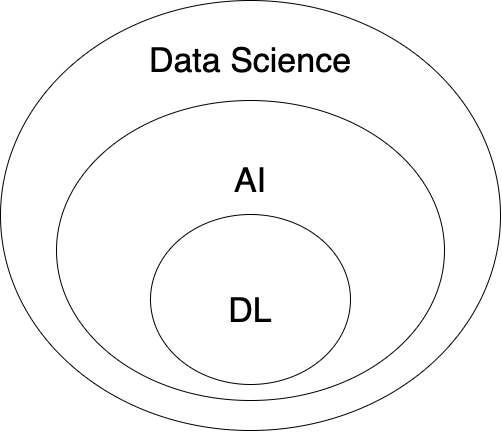
\includegraphics[width=0.8\textwidth]{images/deep-learning}
	\caption{Deep Learning Hirarchy}
	\label{fig:deeplearning}
\end{figure}


Walter Pitts and Warren McCulloch created a computer model based on the neural networks of the human brain\cite{13}. They used a combination of algorithms and mathematics they called “threshold logic” to match the thought process.

Deep learning is a subset of machine learning where artificial neural networks, algorithms inspired by the human brain, learn from large amounts of data\cite{14}. Deep learning allows machines to solve complex problems even when using a data set that is very diverse, unstructured and inter-connected. If there are more than three layers (including input and output) it will qualify as “deep” learning.

Deep learning systems represent the first time computers can understand images at a useful level and reasonable cost. The majority of jobs involve some form of visual perception. ie detection and classification of visual information.

Deep Learning uses a Neural Network to imitate animal intelligence. There are three types of layers of neurons in a neural network: the Input Layer, the Hidden Layer(s), and the Output Layer. Connections between neurons are associated with a weight, dictating the importance of the input value.

Deep learning is a machine learning technique that teaches computers to do what comes naturally to humans. In deep learning, a computer model learns to perform classification tasks directly from images, text, or sound.

Deep learning networks can be successfully applied to big data for knowledge discovery, knowledge application, and knowledge-based prediction. In other words, deep learning can be a powerful engine for producing actionable results

A Deep feature is a consistent response of a node or layer within a hierarchical model to an input that gives a response that's relevant to the model's final output. One feature is considered “deeper” than another depending on how early in the decision tree or other framework the response is activated.

Deep learning is an increasingly popular subset of machine learning. Deep learning models are built using neural networks. A neural network takes in inputs, which are then processed in hidden layers using weights that are adjusted during training. Then the model spits out a prediction. The number of layers of neurons stacked is greater than what's done in Machine Learning, so you now have deep neural networks. Deep Learning is a subset of Machine Learning. Deep learning consists of neural networks with many hidden layers which makes the layers deep. Deep learning then can be defined as neural networks with a large number of parameters.

The layers in one of four fundamental network architectures\cite{15}:
\begin{itemize}

\item Unsupervised Pre-trained Networks.
\item Convolutional Neural Networks.
\item Recurrent Neural Networks.
\item Recursive Neural Networks.
\end{itemize}
Deep learning architectures such as deep neural networks, deep belief networks, recurrent neural networks and convolutional neural networks have been applied to fields including computer vision, speech recognition, natural language processing, audio recognition, social network filtering, machine translation. Its applications are used in industries from automated driving to medical devices. Automated Driving: Automotive researchers are using deep learning to automatically detect objects such as stop signs and traffic lights. In addition, deep learning is used to detect pedestrians, which helps decrease accidents. he 'deep' in deep learning simply refers to having multiple 'hidden' layers; that is layers that aren't the input, or the final output, but somewhere in between.

One of the Deep learning algorithm CNN is suitable for spatial data such as images\cite{16}. RNN is suitable for temporal data, also called sequential data\cite{17}. CNN is considered to be more powerful than RNN. They unlike feed-forward neural networks - can use their internal memory to process arbitrary sequences of inputs.

More layers can be better but also harder to train. As adding a second layer only improves the accuracy by approx 0.2\% (0.9807 vs. 0.9819) after 10 epochs.

Long short-term memory (LSTM) is an artificial recurrent neural network (RNN) architecture used in the field of deep learning\cite{18}. LSTM networks are well-suited to classifying, processing and making predictions based on time series data since there can be lags of unknown duration between important events in a time series.

Human mankind always wanted to have the machines which would have the ability to do the reasoning aspect by it itself. Building such a intellectual machine which could do all reasoning work by itself was a big challenge. Having a machine which could function like a human brain and have the capacity to do the logical operations all by itself was huge challenge. A machine which could actually behave like a human brain. Well, that desire of human mankind to have such a computing machine lead to emergence of the concept of AI i.e artificial intelligence. AI is a concept which acted as a great tool to give a huge strength to the computing machines these days. AI has a capacity to work exactly like how human neural system work. Well, the alogrithum used to design any AI concept was inspired by human neural system.

\begin{figure}[ht]
	\centering
	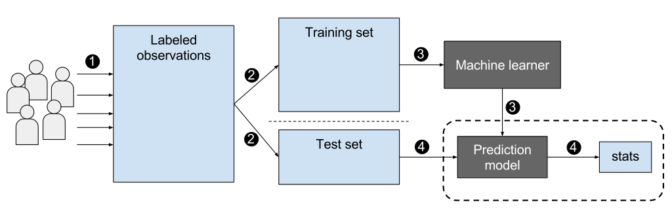
\includegraphics[width=0.8\textwidth]{images/supervised-machine-learning.png}
	\caption{Supervised Machine Learning}
	\label{fig:supervised-machine-learning}
\end{figure}


As the research progressed in the field of AI which lead to have remarkably improved piece of technology , the concept of machine learning came into existence alongside with all of this. Machine learning is an important part of AI.machine learning is a concept where the machine has the capacity to learn by itself from the given set of data in a particular manner.

% \begin{figure}[ht]
% 	\centering
% 	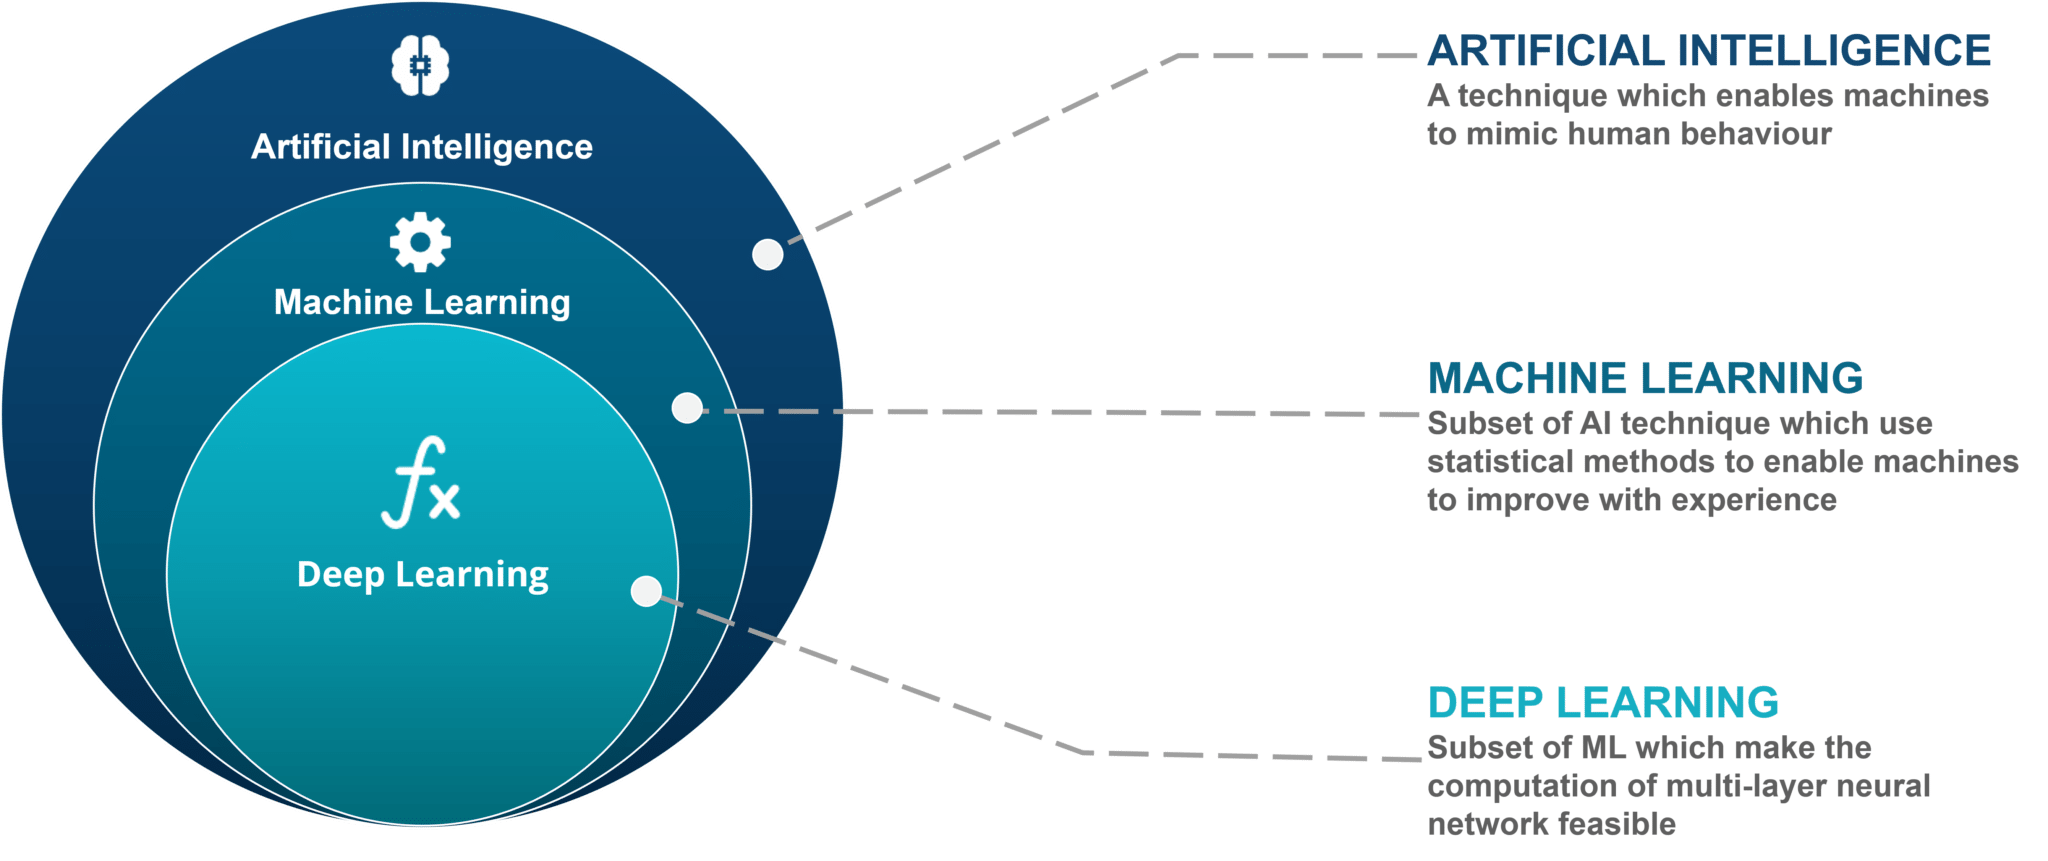
\includegraphics[width=0.8\textwidth]{images/classification-of-ai.png}
% 	\caption{Classification of AI}
% 	\label{fig:classification-of-ai}
% \end{figure}

Earlier the information stored in the system and how the system used to work was based on hard core computational language. The language was more in the numeric form which not giving the freedome of any other sort of interpretation. The language used for these machinery was more scientific. To have a reasoning capability in the machine, there was a huge need of thee development of some different sort of language system. Due to this need, the concept of AI came into existence.

AI gave the computers the reasoning ability and analyise the data using thise reasoning logics.

But later feeding the data everytime to the syste to check the result became a proble. So as to solve such problem, people needed something which could actually self learn the data around the world. So as to accomplish that task, the concept of machine learning came ino existence. Where the concept of machine learning opened the gateway for the machine to self identify and learn from the data available to  them by them selves and act accurately over it.

\begin{figure}[ht]
	\centering
	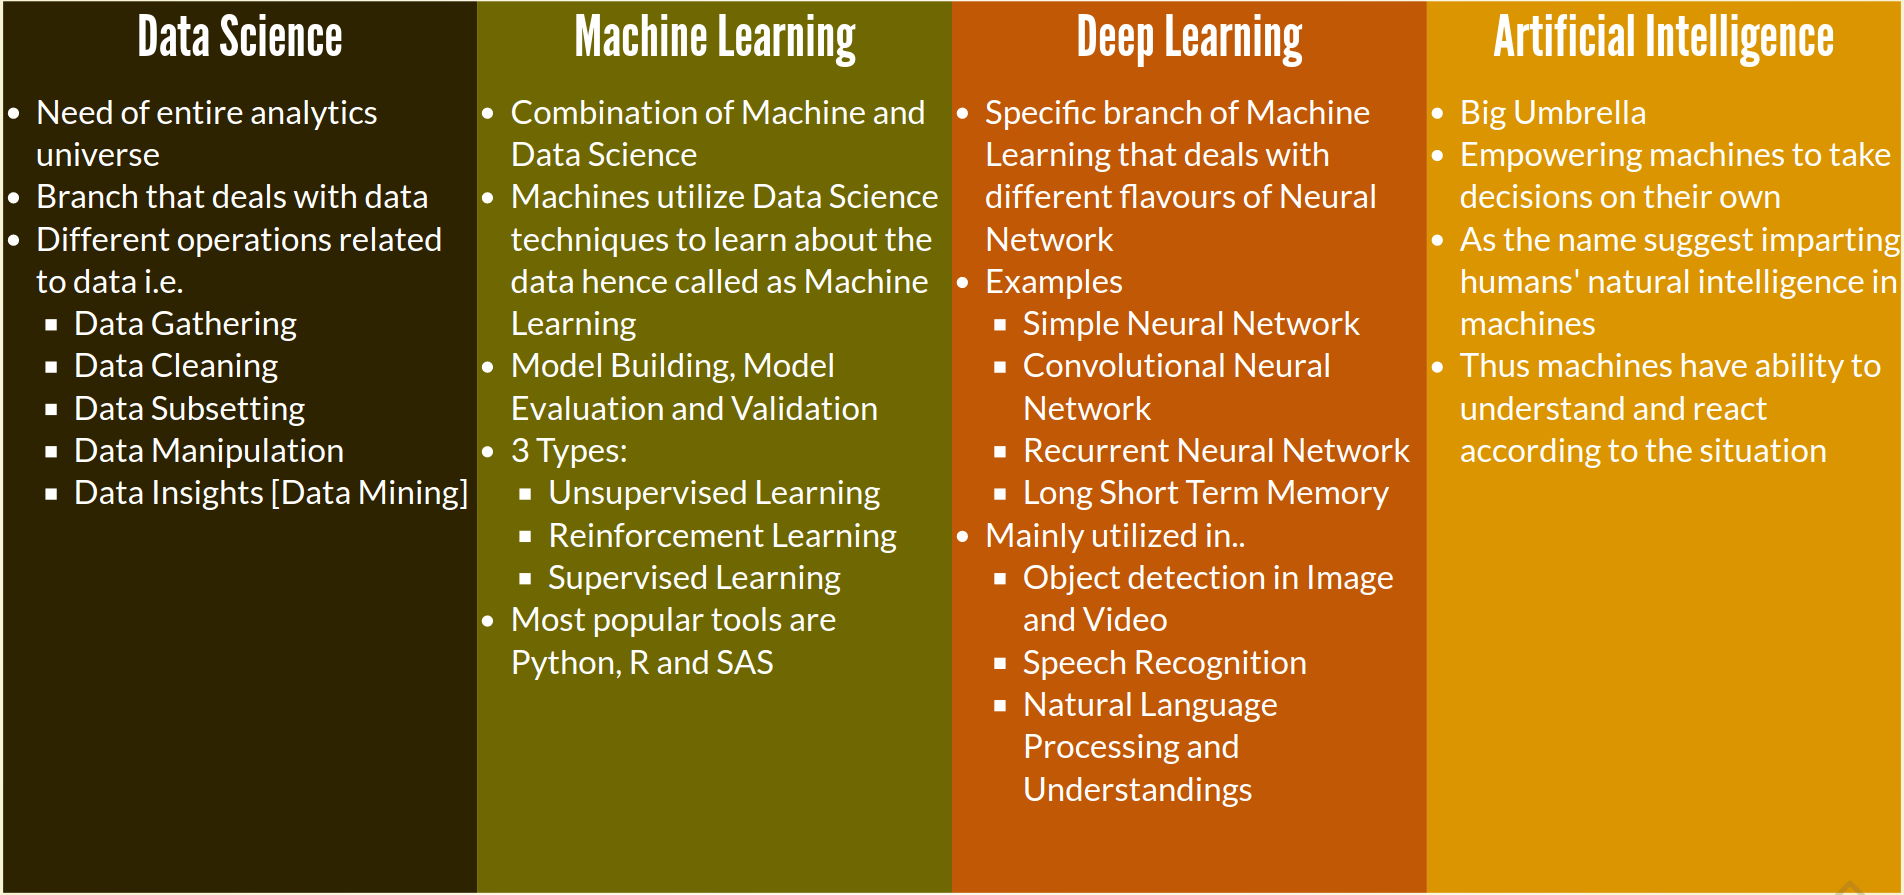
\includegraphics[width=0.8\textwidth]{images/ai.png}
	\caption{Difference between Data Science, ML, DL and, AI }
	\label{fig:ai}
\end{figure}


After this, to solve more complexed problem using AI and using machine learning,  we need more sophisticated tools. From where exactly the concept tof deep learning came into existence. Deep learning is the part of machine learning you can say the eep learning is the subset of the machine learning.

% \begin{figure}[ht]
% 	\centering
% 	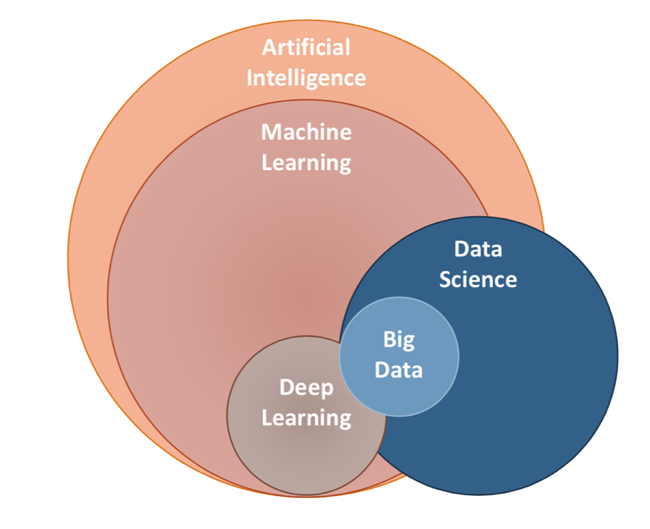
\includegraphics[width=0.8\textwidth]{images/venn-diagram.png}
% 	\caption{Venn Diagram}
% 	\label{fig:venn}
% \end{figure}

Deep learning is majorly used to interpret the data and come up with the conclusions where there is huge lack of segregated data. Where the data available to us is not in a presentable format and completely unorganized, there deep learning act a strong tool to do our analysis over those type of data and retrieve something valuable out of it



\section{Transfer Learning}

Transfer learning (TL) is a research problem in machine learning (ML) that focuses on storing knowledge gained while solving one problem and applying it to a different but related problem\cite{19}. For example, knowledge gained while learning to recognize cats could apply when trying to recognize tigers. This area of research bears some relation to the long history of psychological literature on transfer of learning but from the practical standpoint, reusing or transferring information from previously learned tasks for the learning of new tasks has the potential to significantly improve the sample efficiency of a reinforcement learning agent.

Algorithms are available for transfer learning in Markov logic networks and Bayesian networks. Transfer learning has also been applied to cancer subtype discovery, general game playing, text classification, digit recognition and spam filtering.

In 2020 it was discovered that, due to their similar physical natures, transfer learning is possible between Electromyographic (EMG) signals from the muscles when classifying the behaviours of Electroencephalographic (EEG) brainwaves from the gesture recognition domain to the mental state recognition domain\cite{20}. It was also noted that this relationship worked vice-versa, showing that EEG can likewise be used to classify EMG in addition. The experiments noted that the accuracy of neural networks and convolutional neural networks were improved through transfer learning both at the first epoch and at the asymptote.So algorithms are improved by exposure to another domain.

The main features are: What transfer learning is and how to use it. Common examples of transfer learning in deep learning.When to use transfer learning on your own predictive modelling problems.

Transfer learning is related to problems such as multi-task learning and concept drift and is not exclusively an area of study for deep learning. The transfer learning is popular in deep learning given the enormous resources required to train deep learning models or the large and challenging datasets on which deep learning models are trained. Transfer learning is an optimization, a shortcut to saving time or getting better performance. It is not obvious that there will be a benefit to using transfer learning in the domain until after the model has been developed and evaluated. These features  are required for Transfer learning:

Higher start. The initial skill (before refining the model) on the source model is higher than it otherwise would be.
Higher slope. The rate of improvement of skill during the training of the source model is steeper than it otherwise would be.
Higher asymptote. The converged skill of the trained model is better than it otherwise would be.

\textbf{Two models of Transfer Learning}
\begin{itemize}
	\item Develop a Model Approach
	\item Pre-trained Model Approach
\end{itemize}

\textbf{Develop a Model Approach}

\begin{itemize}
\item Select Source Task. You must select a related predictive modelling problem with an abundance of data where there is some relationship in the input data, output data, and/or concepts learned during the mapping from input to output data.
\item Develop Source Model. Next, you must develop a skilful model for this first task. The model must be better than a naive model to ensure that some feature learning has been performed.
\item Reuse Model. The model fit on the source task can then be used as the starting point for a model on the second task of interest. This may involve using all or parts of the model, depending on the modelling technique used.
\item Tune Model. Optionally, the model may need to be adapted or refined on the input-output pair data available for the task of interest.
\end{itemize}

\textbf{Pre-trained Model Approach}
\begin{itemize}
\item \textbf{Select the Source Model.} A pre-trained source model is chosen from available models. Many research institutions release models on large and challenging datasets that may be included in the pool of candidate models from which to choose from.
\item \textbf{Reuse Model.} The model pre-trained model can then be used as the starting point for a model on the second task of interest. This may involve using all or parts of the model, depending on the modelling technique used.
\item \textbf{Tune Model.} Optionally, the model may need to be adapted or refined on the input-output pair data available for the task of interest.
\end{itemize}



Transfer learning is a different type of machine learning method.
As the concept of machine learning is really important to have good AI based programme
and to have good analytical software. As explained in the starting section about the
emergence of machine learning. Elaborating the importance of the machine learning here.

It is very important to understand the kind of technique we are using for the machine
learning process. As the technique we use for the machine learning process plays a very big
part at how quality results we will receive and how fast the execution of the work will take
place.

So there are various type of machine learning techniques in the market.

Where
1. Supervised learning – in this learning the machine learns by flashing the certain set
of information infront of it. It is like learning like a small kid where the kid learns by
having flash cards.

Some common application of supervised learning are as follows :-

Advertisement clickablity
Identification of spam
Facial recoginition




Unsupervised learning –in this sort of learning the machine is feed with unorganised
data. After feeding the system with the unorganized , the system is allowed to
identify the difference among them by itself.

Some common application of unsupervised learning are as follows :-

  Recommendation system
  Buying behaviour
  Common issue rectifier

Reinforcement learning- In this type of learning the machine learn by iterating the
given data again and again. The machine learning by through same type of data
various times and becoming more accurate about it.

Some common application of reinforcment learning are as follows :-

  Video games
  Industrial management
  Management of resources


Here we will talk about following things about transfer learning
	What is exactly transfer learning
	Real time application of transfer learning
	Productivity impact by using transfer learning.

\section{Challenges and Problem Identification}

Limitations in applying the prediction model in the production environment.
\\

1. Sensor nodes are resource constraint so the prediction model cannot be deployed on sensor nodes.

2. Cluster head can have more resources in comparison to the individual nodes but the machine learning model also cannot be applied there because a cluster head needs to process data collected from a number of different sensor nodes, which intern leave no option to deploy on the cluster head.

3. Machine learning algorithm needs heavy computing generally GPUs are used for the training of the machine learning models, and to be applied in the production environment you have to continue training and updating the model to better adapt for the upcoming missing values, so remote devices are not the choice for the deployment.

4. For training a supervised deep-learning algorithm we need a huge amount of labeled data, which is rare in the IoT and WSN environment.


\section{Motivation}

Cloud computing is a branch of computer science where a network of computers connected to the internet (called cloud) and available for use as per demand.


As there is no limitation in the computing capacity and resources in the cloud and IoT devices are connected to the internet the IoT devices can send their data to these cloud in real-time for processing and get a response (corrective measure) simultaneously.


\section{Research Objective}
The specific objective of this dissertation are as follows:

1. To find an approach to apply deep learning for imputing missing time series data generated by wireless sensor network and also for time series forecasting when there is a scarcity of data produced by the wireless sensor network. \\

2. Applying and studying different deep learning algorithm for time series imputation and forecasting in wireless sensor network. \\

% \noindent
3. Applying transfer learning in wireless sensor network and study the improvement. \\

\section{Methodology}
To complete this task the jupyter (a free and open source integrated developement environment (IDE) is being used for python). The resutls have been obtained by a set of code containing predefined functions in various packages or libraries available in python.


\section{Thesis Organisation}
This thesis consists of 6 chapters. Inside the Chapter 1 an overview of machine learning, wireless sensor network, transfer learning followed by problem statement and research objective. Chapter 2 consists of related work in this field. Chapter 3 and 4 explains the various steps which make up the proposed mechanism. Chapter 5 presents the results and analysis of the proposed model followed by conclusion and future scope.

\section{Summary}
In this chapter various component of machine learning, transfer learning, deep learning and wireless sensor network are discussed. 
Various challenges are also identified in this chapter.

In the next chapter various different literature present on this topic are aggregated.
